记录上一个访问的边时要记录边的编号,不能记录上一个过来的节点(因为会有重边)!!!

(如果选择在加边的时候特判,注意编号问题:用输入顺序来对应数组中位置的时候,重边跳过,但是需要 tot+=2。)

圆方树示意图:

\begin{figure}[H]
    \centering
    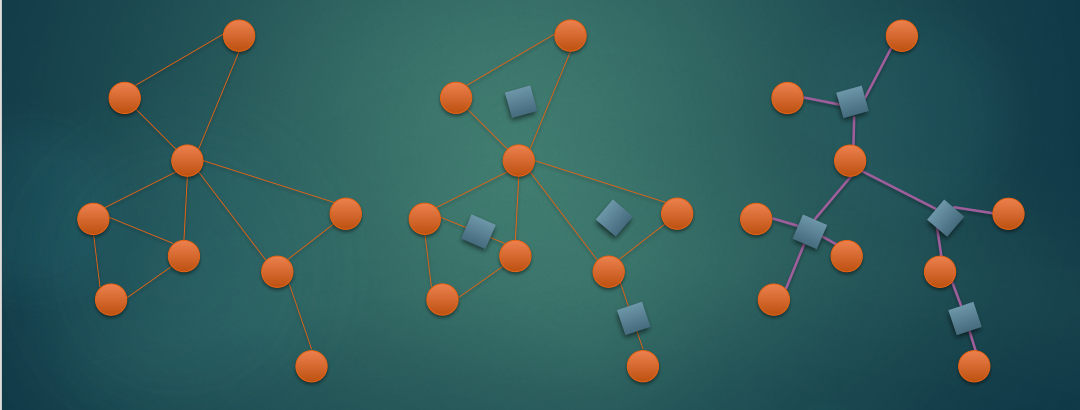
\includegraphics[width=0.45\textwidth]{src/graph/tarjan-tree.png}
    \caption{圆方树示意图}
\end{figure}

\begin{minted}{cpp}
/*** 缩点 ***/
// 找出强联通分量后,对每一条边查看是否在同一个 scc 中,如果不在就加边
void tarjan(int x)
{
	dfn[x]=low[x]=++Time,sta[++tp]=x,ins[x]=true;
	for(int i=hea[x];i;i=nex[i])
	{
		if(!dfn[ver[i]]) tarjan(ver[i]),low[x]=min(low[x],low[ver[i]]);
		else if(ins[ver[i]]) low[x]=min(low[x],dfn[ver[i]]);
	}
	if(dfn[x]==low[x])
	{
        scc++;
		do { x=sta[tp],tp--,ins[x]=false,bel[x]=scc; }
        while (dfn[x]!=low[x]);
	}
}
/*** 割点 ***/
void tarjan(int x,int Last)
// Last 是边的编号,tot 初始值为 1,i 与 i^1 互为反边
{
    dfn[x]=low[x]=++Time;
    for(int i=hea[x];i;i=nex[i])
    {
        if(!dfn[ver[i]])
        {
            tarjan(ver[i],i),low[x]=min(low[x],low[ver[i]]);
            if(low[ver[i]]>dfn[x]) edg[i]=edg[i^1]=true;
        }
        else if(dfn[ver[i]]<dfn[x] && i!=(Last^1)) low[x]=min(low[x],dfn[ver[i]]);
    }
}
/*** 圆方树、点双 ***/
// G 表示原图,T 是新建的圆方树
// 一条边也是点双
// 圆方树只存在圆 - 方边!!!
int Time,dfn[N],low[N],sta[N],siz[N];
vector<int> G[N],T[N<<1]; // 不要忘记给数组开两倍
void tarjan(int u)
{
    dfn[u]=low[u]=++Time,sta[++tp]=u;
    for(int v:G[u])
    {
        if(!dfn[v])
        {
            tarjan(v),low[u]=min(low[u],low[v]);
            // 这里对 low[v]>=dfn[u] 进行计数,根节点需要 2 个,其他节点需要 1 个,那么就是割点。
            if(low[v]==dfn[u])
            {
                int hav=0; ++All;
                for(int x=0;x!=v;tp--) x=sta[tp],T[x].pb(All),T[All].pb(x),hav++;
                T[u].pb(All),T[All].pb(u);
                siz[All]=++hav;
            }
        }
        else low[u]=min(low[u],dfn[v]);
    }
}
\end{minted}